\documentclass[11pt,twocolumn]{amsart} % twocolumn
\usepackage{geometry}                % See geometry.pdf to learn the layout options. There are lots.
\geometry{a4paper}                   % ... or a4paper or a5paper or ... 
%\geometry{landscape}                % Activate rotated page geometry
%\usepackage[parfill]{parskip}    % Activate to begin paragraphs with an empty line rather than an indent
\usepackage{graphicx}
\usepackage{amssymb}
\usepackage{epstopdf}
\DeclareGraphicsRule{.tif}{png}{.png}{`convert #1 `dirname #1`/`basename #1 .tif`.png}


\title{Some stuff for Rubyk}
\author{Gaspard Buma}
%\date{}                                           % Activate to display a given date or no date

\begin{document}

\twocolumn[
\maketitle
]
\section{Variance of a value}

The \textbf{variance} (expressed with the symbol $\sigma^2$ or $\sigma_S^2$) measures the dispersion of a set of values $\textbf{S}$ from the mean value $\mu$ or expected value $E(\textbf{S})$. The mean value is~:
\begin{equation*}
  \mu = E(\textbf{S}) = \frac{1}{l} \sum_1^{l} s_l
\end{equation*}

$l$ being the number of elements in the set. The variance can be computed as~:
\[
  \sigma^2 = E[(\textbf{S} - \mu)(\textbf{S} - \mu)] = \frac{1}{l} \sum_1^{l} (s_l - \mu)^2
\]

For example, given the set of values $\textbf{S} = [1,4,3,6]$, the mean value $\mu$ is~:
\[
  \mu = \frac{1+4+3+6}{4} = 3.5,
\]

and the variance $\sigma^2$~:
\begin{align*}
  \sigma^2 = & (1-3.5)^2 + (4-3.5)^2 +\\
             & \frac{(3-3.5)^2 + (6-3.5)^2}{4} = \frac{13}{4} = 3.25
\end{align*}

\section{variance-covariance matrix}

The \textbf{variance-covariance matrix} is the generalisation to greater dimensions of the variance seen before. Imagine we have a set $\textbf{S}$ of vectors of dimension $n$ and we want to compute the variance of these vectors. We must first compute the expected value $E(\textbf{S})$ which is the mean vector $\mu$~:
\begin{align*}
  E(\textbf{S}) = & \vec{\mu} = \begin{bmatrix} \mu_1, \hdots, \mu_n \end{bmatrix} \\
       = & \frac{1}{l} \begin{bmatrix} \begin{bmatrix} s_{1,1}, \hdots, s_{1,n} \end{bmatrix} \\ + \\ \vdots \\ + \\ \begin{bmatrix} s_{l,1}, \hdots, s_{l,n} \end{bmatrix} \end{bmatrix}
\end{align*}

We can build a matrix $\Theta$ (theta) of size ($l,n$) from the vector $\mu$ (mu)~:
\begin{equation*}
  \Theta = \begin{bmatrix} \vec{\mu} \\ \vdots \\ \vec{\mu} \end{bmatrix}
\end{equation*}

From the definition of the variance, we have
\begin{equation*}
  \Sigma = E \begin{bmatrix} (\textbf{S} - \Theta)^T (\textbf{S} - \Theta)\end{bmatrix}
\end{equation*}

thus each entry in the variance-covariance matrix $\Sigma$ (sigma) is~:
\begin{equation*}
  \Sigma_{ij} = \frac{\sum_{k=1}^{l} (s_{ki} - \mu_i)(s_{kj} - \mu_j)}{l}.
\end{equation*}


For example, given the set $\textbf{S}$ formed with three experiments measuring two values~:
\begin{displaymath}
  \textbf{S} = \begin{bmatrix} 1 & 1 \\ 0 & 4 \\ 2 & 1 \end{bmatrix},
\end{displaymath}

we can compute the expected value~:
\begin{equation*}
  \vec{\mu} = \frac{1}{3} \begin{bmatrix} \left( \begin{array}{c} 1 \\ + \\ 0 \\ + \\ 2 \end{array} \right) \left( \begin{array}{c} 1 \\ + \\ 4 \\ + \\ 1 \end{array} \right) \end{bmatrix} = \begin{bmatrix} 1 & 2 \end{bmatrix}.
\end{equation*}


To find variance-covariance matrix, let us first compute the \emph{mean deviation form} of $\textbf{S}$~:
\begin{equation*}
  \textbf{T} = \textbf{S} - \Theta = \begin{bmatrix} (1-1) & (1-2) \\ (0-1) & (4-2) \\ (2-1) & (1-2)\end{bmatrix} = \begin{bmatrix} 0 & -1 \\ -1 & 2 \\ 1 & -1\end{bmatrix}.
\end{equation*}

We can now find $\Sigma$~:
\begin{align*}
  \Sigma = & E \begin{bmatrix} \textbf{T}^T\textbf{T}\end{bmatrix} = \frac{1}{n-1} \begin{bmatrix} \textbf{T}^T\textbf{T}\end{bmatrix} \\
         = & E \begin{bmatrix} \begin{bmatrix} 0 & -1 & 1 \\ -1 & 2 & -1\end{bmatrix} \begin{bmatrix} 0 & -1 \\ -1 & 2 \\ 1 & -1\end{bmatrix} \end{bmatrix} \\
         = & E \begin{bmatrix} 0*0 + -1*-1 + 1*1 & \hdots \\ -1*0 + 2*-1 + -1*1 & \hdots \end{bmatrix} \\
         = & E \begin{bmatrix} 2 & -3 \\ -3 & 6 \end{bmatrix} = \frac{1}{2} \begin{bmatrix} 2 & -3 \\ -3 & 6 \end{bmatrix}
         = \begin{bmatrix} 1 & -\frac{3}{2} \\ -\frac{3}{2} & 3\end{bmatrix}
\end{align*}

From the result above, $1$ is the variance along $x$, $3$ is the variance along $y$ and $-\frac{3}{2}$ is the covariance between the two dimensions. There are proofs on why we should use $\frac{1}{n-1}$ for the correct normalization factor instead of the straight-forward $\frac{1}{n}$ but this is beyond the scope of my competences...

\section{Mahalanobis distance}

Let us compute the \textbf{Mahalanobis distance} from a vector $\vec{t}$ to the set $\textbf{S}$ with the variance-covariance matrix $\Sigma$ and the mean value $\vec{\mu}$~:
\begin{equation*}
  D_M(\vec{t}) = \sqrt{(\vec{t} - \vec{\mu})\Sigma^{-1}(\vec{t} - \vec{\mu})^T}
\end{equation*}

If we remove the covariances from the matrix $\Sigma$, we have a diagonal matrix whose entries are the variances (standard deviations) for each dimension ($1$ and $3$ in the example above). The Mahalanobis distance becomes the \textbf{normalized Euclidean distance}~:
\begin{equation*}
  D_{nE}(\vec{t}) = \sqrt{\sum_{i=1}^{n}\frac{(t_i - \mu_i)^2}{\sigma_i^2}}.
\end{equation*}

From the example we used above we compute the different distances for two vectors $\vec{t_1}$ and $\vec{t_2}$~:

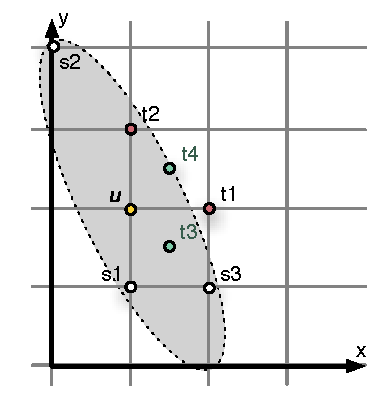
\includegraphics{points.pdf}
\begin{align*}
  \vec{t_1}  = & \begin{bmatrix} 2 & 2 \end{bmatrix} \\
  \vec{t_2}  = & \begin{bmatrix} 1 & 3 \end{bmatrix} \\
  \vec{\mu} = & \begin{bmatrix} 1 & 2 \end{bmatrix} \\
  \Sigma    = & \begin{bmatrix} 1 & -\frac{3}{2} \\ -\frac{3}{2} & 3\end{bmatrix}
\end{align*}

The \textbf{Euclidean distance} $d$ is the same for both points, even though it is visible that $\vec{t_1}$ is more ``out of the way" then $\vec{t_2}$ ~:
\begin{align*}
  d_1 = & \sqrt{\sum_{i=1}^{n}(t_i - \mu_i)^2} \\
     = & \sqrt{(2-1)^2 + (2-2)^2} = 1 \\
  d_2 = & \sqrt{(1-1)^2 + (3-2)^2} = 1
\end{align*}

The \textbf{normalized Euclidean distance} $d_{nE}$ should show that $\vec{t_2}$ matches the set $\textbf{S}$ better then $\vec{t_1}$~:
\begin{align*}
  d_{1nE} = & \sqrt{\frac{(2-1)^2}{1} + \frac{(2-2)^2}{3}} = 1 \\
  d_{2nE} = & \sqrt{\frac{(1-1)^2}{1} + \frac{(3-2)^2}{3}} = \frac{1}{\sqrt{3}} \approx 0.6.
\end{align*}

This is better. We can see that $\vec{t_1}$ is penalized for being out of the way in the wrong direction. The ``penalty" for being badly adjusted along the $x$ axis is $1$ when it is only $\frac{1}{3}$ along the $y$ axis.

Let's now see what the Mahalanobis distance tells us. First we need to compute $\Sigma^{-1}$~:
\begin{equation*}
  \Sigma^{-1} = \frac{1}{(1*3 - -\frac{3}{2}*-\frac{3}{2})} \begin{bmatrix} 3 & \frac{3}{2} \\ \frac{3}{2} & 1\end{bmatrix} = \begin{bmatrix} 4 & 2 \\ 2 & \frac{4}{3} \end{bmatrix}
\end{equation*}

We can now find the distances~:
\begin{align*}
  d_{1M} = & \sqrt{(\vec{t_1} - \vec{\mu})\Sigma^{-1}(\vec{t_1} - \vec{\mu})^T} \\
         = & \sqrt{\begin{bmatrix} 1 & 0 \end{bmatrix} \begin{bmatrix} 4 & 2 \\ 2 & \frac{4}{3}\end{bmatrix} \begin{bmatrix} 1 \\ 0 \end{bmatrix}} \\
         = & \sqrt{\begin{bmatrix} 4 & 2 \end{bmatrix} \begin{bmatrix} 1 \\ 0 \end{bmatrix}} = 2\\
  d_{2M} = & \sqrt{\begin{bmatrix} 0 & 1 \end{bmatrix} \begin{bmatrix} 4 & 2 \\ 2 & \frac{4}{3}\end{bmatrix} \begin{bmatrix} 0 \\ 1 \end{bmatrix}} \\
         = & \sqrt{\begin{bmatrix} 2 & \frac{4}{3}\end{bmatrix} \begin{bmatrix} 0 \\ 1 \end{bmatrix}} = \frac{2}{\sqrt{3}} \approx 1.2\\
\end{align*}

These distances classify the two vectors in the exactly the same way as the normalized Euclidean distances. Why is that so ? The reason is that our vectors are always away from the mean value in a single direction at a time, thus the ``covariance'' part of the error is never used.

What happens with the two points $\vec{t_3}$ and $\vec{t_4}$ ? From the first look at the picture we can see that their distance to the mean value is the same~:
\begin{align*}
  d_3 = & \frac{1}{\sqrt{2}} \approx 0.7 \\
  d_4 = & \frac{1}{\sqrt{2}} \approx 0.7
\end{align*}

Their normalized Euclidean values are also the same as they differ from the mean value exactly in the same way along $x$ and $y$~:
\begin{align*}
  d_{3nE} = & \frac{1}{\sqrt{3}} \approx 0.6\\
  d_{4nE} = & \frac{1}{\sqrt{3}} \approx 0.6
\end{align*}

Now comes the Mahalanobis distances~:
\begin{align*}
  d_{3M} = & \frac{1}{\sqrt{3}} \approx 0.6\\
  d_{4M} = & \frac{\sqrt{14}}{\sqrt{6}} \approx 1.5
\end{align*}

This type of distance calculation is the only one that reflect the difference between the two vectors $\vec{t_3}$ and $\vec{t_4}$ and classifies $\vec{t_4}$ as beeing further ``away'' then $\vec{t_3}$, like our eyes tell us from a quick look at the picture~!

\section{Eigenvalues}

Before we study \emph{Principal Component Analysis}, we need some understanding of eigenvalues. Imagine we have a transformation matrix \textbf{P}~:
\begin{equation*}
  \textbf{P} = \begin{bmatrix} 1 & 1 \\ 0 & 2 \end{bmatrix}.
\end{equation*}

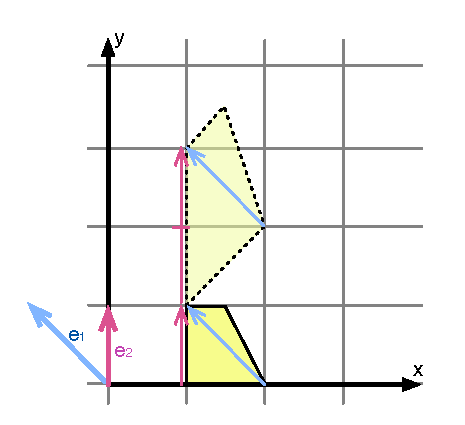
\includegraphics{eigen.pdf}

What are the vectors in this transformation that keep their direction (are not rotated)? Mathematically speaking we want to find $\vec{e}$ such that~:
\begin{equation*}
  \vec{e'} = \vec{e} * \textbf{P} = \lambda \vec{e}
\end{equation*}

We can see from the picture that $\vec{y}$ satisfy this as $\vec{y'}$ is just $2 * \vec{y}$. Such vectors are called \emph{eigenvectors} and their corresponding lambda values \emph{eigenvalues}. To find these vectors, we can rewrite the equation above~:

\begin{equation*}
  \vec{e'} = \vec{e} * \textbf{P} = \lambda \vec{e}
\end{equation*}

as

\begin{equation*}
  \vec{e} * \textbf{P} - \lambda \vec{e} = 0
\end{equation*}

or 

\begin{equation*}
  \vec{e} (\textbf{P} - \lambda \textbf{I}) = 0  
\end{equation*}

We know that an equation of the form~:
\begin{equation*}
  \vec{x} \textbf{A} = 0
\end{equation*}
has only the trivial solution $\vec{x} = \vec{0}$ if the determinant of $\textbf{A}$ is not null. We can therefore find the non-trivial solutions to the equation above by computing the determinant when the latter \emph{is} null. This equation is called the \emph{characteristic equation} of \textbf{P}~:
\begin{equation*}
  det(\textbf{P} - \lambda \textbf{I}) = 0
\end{equation*}

We can now calculate the values of $\lambda$~:
\begin{align*}
  det(\begin{bmatrix} 1 & 1 \\ 0 & 2\end{bmatrix} - \lambda \begin{bmatrix} 1 & 0 \\ 0 & 1 \end{bmatrix}) = & 0 \\
  det(\begin{bmatrix} 1-\lambda & 1 \\ 0 & 2-\lambda\end{bmatrix}) = & 0 \\
  (1-\lambda)(2-\lambda) - 1 * 0 = & 0 \\
  (1-\lambda)(2-\lambda) = & 0
\end{align*}

which has the solutions
\begin{equation*}
\lambda_1 = 1, \lambda_2 = 2
\end{equation*}

The corresponding \emph{eigenvectors} can be found by substituting $\lambda_1$ and $\lambda_2$ in $\vec{e} (\textbf{P} - \lambda \textbf{I}) = \vec{0}$~:
\begin{align*}
  \begin{bmatrix} x & y \end{bmatrix} \begin{bmatrix} 1-\lambda & 1 \\ 0 & 2-\lambda \end{bmatrix} = & 0 \\
  \begin{bmatrix} x_1 & y_1 \end{bmatrix} \begin{bmatrix} 1-1 & 1 \\ 0 & 2-1 \end{bmatrix} = & 0 \\
  \begin{bmatrix} x_1 & y_1 \end{bmatrix} \begin{bmatrix} 0 & 1 \\ 0 & 1 \end{bmatrix} = & 0 \\
  x_1 + y_1 = & 0 \\
  \vec{e_1} = & \begin{bmatrix} t & -t \end{bmatrix}
\end{align*}

and for $\lambda_2$~:
\begin{align*}
  \begin{bmatrix} x_2 & y_2 \end{bmatrix} \begin{bmatrix} 1-2 & 1 \\ 0 & 2-2 \end{bmatrix} = & 0 \\
  \begin{bmatrix} x_2 & y_2 \end{bmatrix} \begin{bmatrix} -1 & 1 \\ 0 & 0 \end{bmatrix} = & 0 \\
  -x_2  = & 0 \\
   x_2  = & 0 \\
  \vec{e_2} = \begin{bmatrix} 0 & t \end{bmatrix} = \vec{y}
\end{align*}

If we look at our transformation picture again, we see that the relation in the direction $\vec{e_1}$ is kept and the relation in the direction of $\vec{e_2}$ is just doubled. This reflects the eigenvalues $1$ and $2$ with the directions of the eigenvectors $\vec{e_1}$ and $\vec{e_2}$.

Before moving on to the following section, we need an important propriety of \emph{symmetric} matrices~: \emph{a symmetric matrix is diagonalized by a matrix of its eigenvectors}. Aouchh, this is a long phrase. In a \emph{symmetric} matrix, all $a_{ij}$ entries are equal to $a_{ji}$ (imagine a mirror across the diagonal of the matrix). To diagonalize a matrix means transform it into another matrix where all entries not on the diagonal are 0 ($a_{ij} = 0\text{ if } i \not= j$) by multiplying it with another matrix. Stated another way, the preceding phrase says that if there is a symmetric matrix \textbf{A}, an invertible matrix \textbf{E} and a diagonal matrix \textbf{D} such that~:
\begin{equation*}
  \textbf{D} = \textbf{E}^{-1}\textbf{A}\textbf{E},
\end{equation*}

then \textbf{E} is a matrix of the \emph{eigenvectors} of \textbf{A}. Is this true ? Why ? First we need to prove that a symmetric matrix is orthogonally diagonizable~:
\begin{equation*}
  
\end{equation*}

\section{Principal Component Analysis}

Principal Component Analysis is a way to extract the ``most proeminent features'' of a data set. It assumes that the data has a good signal to noise ratio which means that \emph{great variance} in the data is a synonym for \emph{relevant feature} and not \emph{big noise}.

In all the calculations below, we need to use the \emph{variations} of the measures. We will thus remove the mean values from our data set and use this new set called the \emph{mean deviation form} of \textbf{S}~:
\begin{equation*}
  \textbf{T} = \textbf{S} - \begin{bmatrix}\vec{\mu} \\ \vdots \\ \vec{\mu}\end{bmatrix}.
\end{equation*}

In order to extract the ``most proeminent features'' of our data, a good idea would be to look at the directions in which the data varies most. Is it along the $\vec{x}$ axis ? The $\vec{y}$ axis ? Somewhere in between ?

Recall from the previous sections that the variance-covariance matrix $\Sigma$ displays variances along the diagonal and covariances off-diagonal. We can use this matrix to extract directions in which the data varies most~:
\begin{equation*}
  \Sigma = \frac{1}{n-1}\textbf{T}^T\textbf{T}.
\end{equation*}

By looking at the diagonals of $\Sigma$, we pick the greatest absolute value and there we are, we found our direction ($3 \Rightarrow \vec{y}$). Is that it ? No, this solution misses the fact that the main direction might not follow one of the axis (dimension) of our recorded data (the ellipsoid is not vertical nor horizontal). What we need is to apply a transformation (rotation + stretch) to our data \textbf{T} into an new basis \textbf{P} prior to looking at the variance-covariance matrix, so that the principal components align with the new basis' axis.
\begin{align*}
  \textbf{T'} = & \textbf{T}\textbf{P} \\
  \Sigma'     = & \frac{1}{n-1}\textbf{T'}^T\textbf{T'}
\end{align*}

Our goal is thus to find a new basis \textbf{P} that gives us great absolute values along the diagonals of $\Sigma'$ and small absolute values off-diagonal (small redundancy). If possible, it would be great to see large variances along the top of the diagonal which would mean we could just cut off the rightmost part of the matrix \textbf{T'} and still have most of the information on the varying signal. To summarize~:
\begin{itemize}
  \item Find a new basis \textbf{P} that reduces the redundancy of the signals (low covariance).
  \item The $\Sigma'$ matrix for \textbf{T'} should ideally be a diagonal matrix with very high values at the top and very small at the bottom, thus showing signals in the first dimensions and pure noise in the last ones.
  \item We could then choose to remove the columns of \textbf{T'} that have greater indices than the number of dimensions we want to keep thus reducing the dimensionality of our data.
\end{itemize}

A simple way to find the solution would be~:
\begin{enumerate}
  \item Find the direction $\vec{e_1}$ that shows the greatest variance in the data \textbf{T}. Normalize this vector. This is our first basis vector.
  \item Find another normalized vector showing the greatest variance that is orthogonal to those already found ($\forall \vec{b}\in \{\text{found vectors}\}, \vec{e_n} \perp \vec{b}$).
  \item Repeat until we have $n$ basis vectors ($n$ is the size of vector space).
\end{enumerate}

The resulting ordered set of vectors are the \emph{principal components} of our data set \textbf{T}.

\section{computing PCA}



\section{applying PCA to \textbf{S}}

Using the same sample data as above, we imagine that the set of points $\textbf{S}$ represents the measures of a moving element. The object actually moves only along the ellipsoid axis $\vec{e} = (-1,2)$, the deviations from this axis is just noise. The goal of PCA is to re-express our set of data in a new basis that reflects this behaviour (data along $\vec{e}$, noise along the other direction). The naive basis (in which we recorded the data) is~:
\begin{equation*}
  \textbf{B} = \begin{bmatrix} \vec{x} \\ \vec{y} \end{bmatrix} = \begin{bmatrix} 1 & 0 \\ 0 & 1 \end{bmatrix} = \textbf{I}
\end{equation*}

We will use PCA to find a new basis $\textbf{P}$ that is a linear combination of the original matrix $\textbf{B}$ and in which we will only look at the data along the greatest axis of the ellipsoid (where the data exhibits the greatest variance). In this new basis, the set of data \textbf{B} becomes~:
\begin{equation*}
  \textbf{S'} = \textbf{S}\textbf{P}
\end{equation*}

The new basis should optimise signal to noise ratio if we consider the first dimension as representing the signal and the second the noise~:
\begin{equation*}
  SNR = \frac{\sigma_{signal}^2}{\sigma_{noise}^2}
\end{equation*}

Before delving any further, we must first transform our data into its \emph{mean deviation form} $\textbf{T}$. 
\begin{equation*}
  \textbf{T} = \textbf{S} - \begin{bmatrix}\vec{\mu} \\ \vdots \\ \vec{\mu}\end{bmatrix} = \begin{bmatrix} 0 & -1 \\ -1 & 2 \\ 1 & -1\end{bmatrix}.
\end{equation*}

We can now easily compute the actual SNR~:
\begin{equation*}
  SNR = \frac{\sum_{k=1}^l T_{k1}^2}{\sum_{k=1}^l T_{k2}^2} = \frac{0+1+1}{1+4+1} = \frac{1}{3}
\end{equation*}

How do we find the new basis that gives us the greatest SNR ? Expressed in another way, we could say~: how do we find the basis that shows greatest variance in the first dimension and mostly noise in the second ?

\section{notes on PCA}

For a deaper understanding of PCA and it's limits, one may have a look at~:
\begin{itemize}
  \item \emph{kernel PCA} to apply a non-linear filtre prior to applying PCA for problems where linearity is an issue.
  \item \emph{ICA} for sets of data whose distribution probabilities are not exponential (Gaussian, Exponential, etc).
  \item \emph{Central Limit Theorem} on why PCA should work most of the time in real world as probabilities usually \textbf{are} gaussian.
\end{itemize}

\onecolumn

\section{Ruby code}
\subsection{variance}
\begin{verbatim}
set   = [1,4,3,6]
mu    = set.inject(0) {|s,v| s + v } / set.size.to_f
sigma = set.inject(0) {|s,v| s + ((v - mu)**2) } / set.size.to_f
\end{verbatim}

\subsection{Mahalanobis distance}
\begin{verbatim}
class Array
  # transpose
  def t
    cols = []
    self[0].each_index do |i|
      cols[i] = map {|v| v[i]}
    end
    cols
  end

  def *(m)
    res = []
    each_index do |row|
      res[row] = []
      m[0].each_index do |col|
        res[row][col] = 0
        self[0].each_index do |i|
          res[row][col] += self[row][i] * m[i][col]
        end
      end
    end
    res
  end

  def det
    (self[0][0] * self[1][1]) - (self[1][0] * self[0][1])
  end

  def /(scalar)
    map {|row| row.map {|v| v / scalar}}
  end

  # vector substraction
  def -(v)
    res = [[]]
    self[0].each_index {|i| res[0][i] = self[0][i] - v[0][i]}
    res
  end

  def to_s
    if self.size > 1 || self[0].size > 1
      if self.size == 1
        row_format = '[' + (" %3.1f" * self[0].size) + " ]\n"
      else
        row_format = '|' + (" %3.1f" * self[0].size) + " |\n"
      end
      self.inject("") {|s,row| s + sprintf(row_format, *row)}
    else
      self[0][0].to_s
    end
  end

  def map_index(&block)
    res = []
    self.each_index do |i|
      res[i] = yield(i,self[i])
    end
    res
  end
end


set = [[1,1],
       [0,4],
       [2,1]]
# mean vector mu
mu = [[]]
set[0].each_index do |i|
  mu[0][i] = set.inject(0) {|s,v| s + v[i] } / set.size.to_f
end

# set - mu
s_mu = set.map do |v|
  r = []
  v.each_index do |i|
    r[i] = v[i] - mu[0][i]
  end
  r
end

# variance-covariance matrix
sigma = (s_mu.t * s_mu) / (set.size - 1.0).to_f

# inverse of sigma
if sigma.det == 0
  puts "Matrix not invertible"
  return
end

# invers of sigma (only for a 2x2 matrix)
sigma_inv = [[  sigma[1][1], -sigma[0][1] ],
             [ -sigma[1][0],  sigma[0][0] ]] / sigma.det

puts "Sigma\n\n"
puts sigma.to_s
puts "\nSigma's inverse\n\n"
puts sigma_inv.to_s

puts "\n\nAll results express value^2 (before square root)"

[
[[[2  , 2  ]],
[ [1  , 3  ]]],
[[[1.5, 1.5]],
[ [1.5, 2.5]]]
].each do |t1,t2|
  puts "\n-----------------------------"
  puts "t1   = #{t1}"
  puts "t2   = #{t2}"
  puts "t1-u = #{t1 - mu}"
  puts "t2-u = #{t2 - mu}\n\n"

  d1 = (t1 - mu).flatten.inject(0) {|s,v| s + v**2} 
  d2 = (t2 - mu).flatten.inject(0) {|s,v| s + v**2}

  puts "d1   = #{d1}"
  puts "d2   = #{d2}\n\n"

  d1nE = (t1 - mu).flatten.map_index{|i,v| v**2 / sigma[i][i] }.inject(0) {|s,v| s + v } 
  d2nE = (t2 - mu).flatten.map_index{|i,v| v**2 / sigma[i][i] }.inject(0) {|s,v| s + v } 

  puts "d1nE = #{d1nE}"
  puts "d2nE = #{d2nE}\n\n"

  d1M = (t1 - mu) * sigma_inv * (t1 - mu).t
  d2M = (t2 - mu) * sigma_inv * (t2 - mu).t

  puts "d1M  = #{d1M}"
  puts "d2M  = #{d2M}\n\n"
end
\end{verbatim}
\end{document}